\section{Resultate \& Ausblick}\label{sec:conflict}

Nachfolgend vergleicht man die drei Dimensionen für die drei verschiedenen Szenarien.

\paragraph{Umwelt}
Die weltweite Nutzung von Tantal bewerten wir für das Jahr 2013 aus ökologischer
Sicht als neutral (5 auf der Skala). Dabei heben sich die geringen direkten
Folgen der Tantalgewinnung und die gravierenden Konsequenzen für den Naturraum
auf, während der Verbrauch als solches ebenfalls als neutral eingeschätzt wird.
Bei einem anhaltenden Trend und der damit einhergehenden Steigerung der
Fördermenge verschlechtern sich die Werte der einzelnen Indikatoren bis 2035 zum
Teil massiv. Speziell der Rohstoffverbrauch und die daraus resultierende
Verminderung des Rohstoffbestandes haben schwerwiegende Folgen. Durch die
Einführung einer neuen Technologie zur Herstellung von Kondensatoren könnte die
Nachfrage hochgerechnet um 40\% gesenkt werden. Da jedoch davon ausgegangen
wird, dass bis 2035 mehr als doppelt so viel Tantal benötigt wird, reicht
diese Massnahme alleine nicht, um zumindest auf dem gleichen Niveau zu bleiben
wie 2013. 
\begin{center}
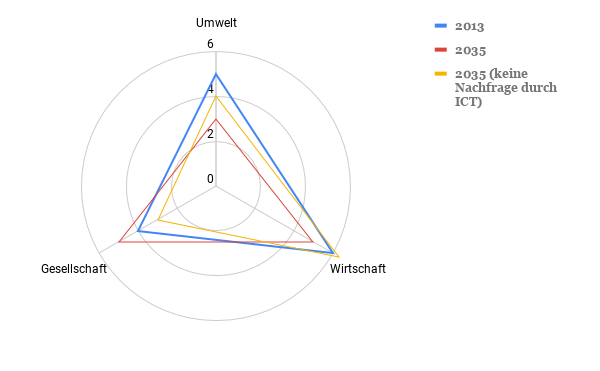
\includegraphics[width=14cm]{images/tantal-results}
\captionof{figure}{Vergleich der Nachhaltigkeit der drei verschiedenen Szenarien.}
\end{center}
